\section{MVC}
\label{ch:mvc}

\subsection{Une structure}


Le secret pour faire de grande applications JavaScript n’est pas de faire une grosse applications JavaScript. Mais plutôt de dissocier votre application dans une série de composants relativement indépendants. Les développeurs font bien souvent l’erreur de créer des applications avec beaucoup d’interdépendances, avec d’énormes fichiers JavaScript linéaires générant une flopée de balises HTML. Ces applications sont difficiles à maintenir et à étendre, et par conséquent devraient être évité à tout prix.

Faire un peu attention à la structure de l'application lorsque vous commencez à la construire peut faire une grande différence sur le résultat final. Ignorez toutes les idées préconçues que vous avez sur JavaScript et traitez le comme un langage orienté object. Utilisez les classes, l’héritages, les objets et les modèles de la même façon que vous le feriez avec un autre langage, comme Python ou Ruby. L’architecture est essentielle du coté serveur alors pourquoi ne pas faire la même chose coté client?  L’architecture retenu dans ce mémoire comme dans la plupart des frameworks présenté est l’architecture MVC, une architecture permettant de maintenir et étendre vos applications. Ce modèle s’applique particulièrement bien aux applications JavaScript.

\subsection{Qu’est ce que MVC ?}


MVC est un modèle de conception qui découpe une application en trois parties: les données (Modèle), la couche de présentation (Vue), et la couche d’interaction de l’utilisation (Contrôleur).

En d’autres termes, le flux dévénement est comme ceci:

\begin{enumerate}

  \item
  L’utilisateur interagit avec l’application

  \item
  Le gestionnaire d’évenements déclenche le Controleur

  \item
  Le Controleur demande les données du modèle, qui est envoyé à la Vue.

  \item
  La Vue présente les données à l’utilisateur.

\end{enumerate}

Ou en représentation graphique

\begin{center}
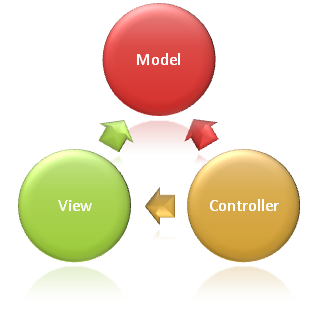
\includegraphics[scale=0.6]{img/mvc.png}
\label{L'architecture MVC}
\end{center}


Le modèle architectural MVC peut même être mis en oeuvre sans bibliothèques ou framework. La clé est de répartir les responsabilités des composants MVC en sections de code défini, en les gardant découpés. Cela permet de rendre indépendant le développement, les tests et la maintenances de chaque composants.



